\chapter{Implementation}
\label{sec:impl}
Reviewernet is a fully client-side application. It builds on a bibliographic dataset extracted from a reference corpus containing more than 180 million records.

The goal is to facilitate a complex process, as the reviewer selection, through multiple and coordinated views about papers and researchers.

In this chapter, we describe our implementation choices, namely: the data and the preprocessing phase, languages, frameworks and external libraries used to deploy the user interface, concluding with an analysis of the code that implements additional features of our interactive visualization system.
\section{The data}
To construct the reference dataset, we collected papers, authors and citations from eight selected sources in the field of Computer Graphics, taken from the Semantic Scholar Research Corpus \cite{ammar:18}. 

The original corpus currently contains more than 180 millions research papers published in all fields, provided as a set of gzipped JSON archives. In Figure \ref{jsonfields} there is the full list of the attributes of a generic record that represents a publication.

\begin{figure}[!ht]
    \centering
    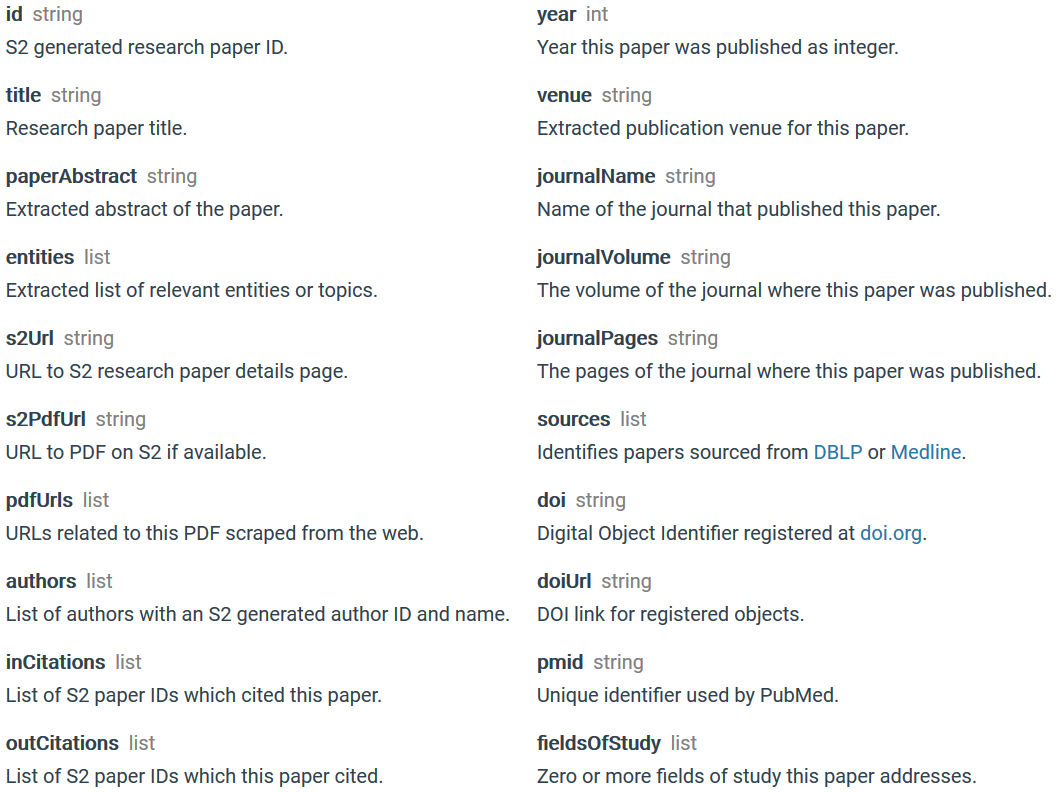
\includegraphics[width=\textwidth]{fig/corpusfields.png}
    \caption{Definition of attributes of the Semantic Scholar coprus.\label{jsonfields}}
\end{figure}

To keep complexity low and offer a cleaner visualization, we filtered the corpus extracting only publications from journals and conference proceedings listed in Table \ref{table:sources}, spanning the years in-between 1995 and 2019. 

The final reference dataset contains 22.887 papers, 145.900 citations, and 29.549 authors.
\begin{table}[!ht]
\renewcommand{\arraystretch}{1.3}
\centering
\begin{tabular}{|l|c|}
\hline
ACM Transactions on Graphics & 2594\\ 
Computer Graphics and Applications  & 1697 \\ 
Computer Graphics Forum & 3521\\ 
Computers \& Graphics & 2092\\ 
IEEE Transactions on Visualization and Computer Graphics & 3638\\ 
Visual Computer & 2107\\ 
Proceedings of IEEE Conference Visualization (pre 2006) & 474 \\ 
Proceedings of ACM SIGGRAPH (pre 2003) & 6718\\
\hline
\end{tabular}
\caption{The selected sources from the Semantic Scholar Research Corpus used in our demonstration scenario. The final reference dataset contains 22.887 papers, 145.900 citations, and 29.549 authors.}
\label{table:sources}
\end{table}

%\input{stats.tex}
\subsection*{Pre-processing}
\label{sec:preproc}

The total size of the corpus is about 180 GB, hence the pre-processing phase is crucial to lower data complexity while maintaining coherence and topic coverage to properly support the reviewer selection process. After non-paper ( such as acknowledgements to reviewers, prefaces, etc.) and useless attributes deletion, each partition has been parsed and filtered separately with a python script. In this filtering step, we use an inexact-search algorithm to correctly assign papers to venues and journals (See Chapter \ref{sec:lang} and \ref{sec:misccode}). Then we have the final consolidation step in which we:
\begin{itemize}
    \item check citations consistency, to ensure we only extract citations published in one of the journals/venues in our reference list (Table \ref{table:sources})
    \item precompute co-authorship relathionships among researchers
    \item merge the filtered data obtaining 3 JSON files (authors, papers, journals) representing the Computer Graphic reference corpus
\end{itemize}

The \emph{papers' file} is a JSON representation of the PN. It contains two lists: \textit{nodes} and \textit{links}, representing respectively papers and citation relathionships. 
\begin{table}[!ht]
    \centering
    \begin{tabular}{ll}
    id {\color[HTML]{656565}string}    & S2 generated paper ID.           \\ 
    value {\color[HTML]{656565}string} & Paper title.                      \\
    year {\color[HTML]{656565}int}     & Publication year of this paper.   \\
    authsId {\color[HTML]{656565}list} & List of S2 generated author IDs.  \\                
    jn {\color[HTML]{656565}string}                                          & Name of the journal that published this paper. \\
    j\_id {\color[HTML]{656565}string}                                        & ID of the journal.                             \\
    venue {\color[HTML]{656565}string}                                       & Extracted publication venue.                   \\
    v\_id {\color[HTML]{656565}string}                                        & Venue ID.                                      \\
    color {\color[HTML]{656565}int}    & Number of in-citations.            \\  
    nOc {\color[HTML]{656565}int} & Number of out-citations. 
\end{tabular}
    \caption{Definition of attributes of the generic node in the PN. \label{tab:nodes}}
   
    \end{table}

    The paper entity is essentialy the same as in the reference corpus with less attributes, as described in Table \ref{tab:nodes}. The link object is simpler: for each citation in the dataset we have the source and target ID and an integer used by the force simultaion algorithm to compute the graph layout. Since the PN layout is static we assign a default value to this field. 
    
    The \emph{authors' file} is a list of JSON, one for each researcher. Table \ref{tab:authors} describes the author entity in ReviewerNet.

\begin{table}[!ht]
    \centering
    \begin{tabular}{ll}
    id {\color[HTML]{656565}string}    & S2 generated researcher ID.           \\ \hline
    value {\color[HTML]{656565}string} & Researcher name.                      \\ \hline
    lastPub {\color[HTML]{656565}list}     & \begin{tabular}[c]{@{}l@{}}List containing the researcher last publication's year\\and S2 ID in the extracted dataset.\end{tabular}\\ \hline
    paperList {\color[HTML]{656565}list} & \begin{tabular}[c]{@{}l@{}}List of papers' IDs authored by this researcher\\in the extracted dataset.\end{tabular}\\    \hline         
    coAuthList {\color[HTML]{656565}dict} & \begin{tabular}[c]{@{}l@{}}A dictionary with one entry for each co-author\\of this researcher. Each dictionary element contains\\pre-computed information about the shared works\\between the two researchers in the extracted dataset. \end{tabular}
\end{tabular}
    \caption{List and description of researchers' attributes in the ReviewerNet representaion. \label{tab:authors}}
   
    \end{table}

The \texttt{coAuthList} field is a fondamental one: it allows to rapidly discover conflicts among researchers, easing the real-time computation load.

The \emph*{journals' file}, eventually, contains information about the journal/venue names consolidation and useful statistics: for each entity we store:
    \begin{itemize}
        \item journal/venue unique ID
        \item a list of names and achronims that refers to the journal/venue; this list is used in the inexact-search routine
        \item the number of papers, authors and citations, collected with the reference list \ref{table:sources}
        \item a pre-computed \emph{journal/venue score}, that is the total number of in-citations, over all the journal/venue publications, coming from a different journal/venue; this score is used to decide in which order the journal/venues will be showed to the user and in the corresponding color-map.  
    \end{itemize}

This file is loaded first once the user choose the instance upon which want to run a ReviewerNet session and is used to quickly print statistics about the instance, without loading the entire dataset.
\section{Languages \& external libraries}
\label{sec:lang}
\begin{itemize}
    \item static UI: HTML5, CSS3, bootstrap
    \item dynamic: JS (JqueryUI for widgets) and D3JS
    \item preproc: Bash and Python (fuzzywuzzy) 
\end{itemize}

\section{Additional features}
\label{sec:misccode}

\begin{itemize}
    \item export/load session snapshot (formato file, spiegare inconsistenza fra id di varie versioni del corpus)
    \item import from biblio \& \texttt{p\_search}
    \item generating a custom reviewernet instance
\end{itemize}